\begin{figure}[htbp]
\centering
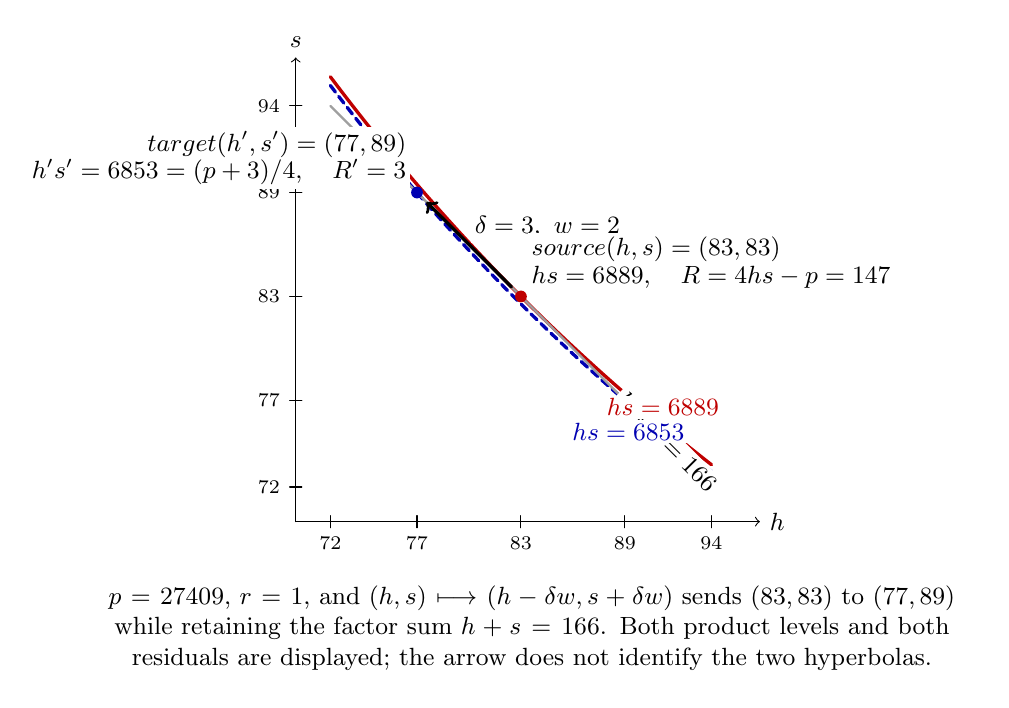
\begin{tikzpicture}[font=\small,line cap=round,line join=round]
  \begin{scope}[x=0.22cm,y=0.22cm,xshift=-15.4cm,yshift=-15.4cm]
    \draw[->] (70,70) -- (96.8,70) node[right] {$h$};
    \draw[->] (70,70) -- (70,96.8) node[above] {$s$};
    \foreach \x in {72,77,83,89,94}{
      \draw (\x,70.35) -- (\x,69.65)
        node[below] {\scriptsize $\x$};
      \draw (70.35,\x) -- (69.65,\x)
        node[left] {\scriptsize $\x$};
    }

    \draw[red!75!black,very thick]
      plot[domain=72:94,samples=100]
      (\x,{6889/\x});
    \draw[blue!70!black,very thick,densely dashed]
      plot[domain=72:94,samples=100]
      (\x,{6853/\x});
    \draw[gray!75,thick]
      plot[domain=72:94,samples=2]
      (\x,{166-\x});

    \fill[red!75!black] (83,83) circle[radius=0.34];
    \fill[blue!70!black] (77,89) circle[radius=0.34];
    \draw[->,black,very thick]
      (82.45,83.55) -- (77.55,88.45)
      node[midway,above right,fill=white,inner sep=1.5pt]
      {$\delta=3,\ w=2$};

    \node[above right,align=left,fill=white,inner sep=1.5pt]
      at (83.35,83.2)
      {$\text{source }(h,s)=(83,83)$\\[-1pt]
       $hs=6889,\quad R=4hs-p=147$};
    \node[above left,align=right,fill=white,inner sep=1.5pt]
      at (76.65,89.15)
      {$\text{target }(h',s')=(77,89)$\\[-1pt]
       $h's'=6853=(p+3)/4,\quad R'=3$};
    \node[rotate=-45,fill=white,inner sep=1pt]
      at (91.4,74.6) {$h+s=166$};
    \node[red!75!black,fill=white,inner sep=1pt]
      at (91.2,76.6) {$hs=6889$};
    \node[blue!70!black,fill=white,inner sep=1pt]
      at (89.2,75.2) {$hs=6853$};
  \end{scope}

  \node[align=center,text width=0.92\linewidth]
    at (3.0,-1.35)
    {$p=27409$, $r=1$, and
     $(h,s)\longmapsto(h-\delta w,s+\delta w)$ sends
     $(83,83)$ to $(77,89)$ while retaining the factor sum $h+s=166$.
     Both product levels and both residuals are displayed; the arrow does not
     identify the two hyperbolas.};
\end{tikzpicture}
\caption{The exact factor-sum arrow
$(h,s)\mapsto(h-\delta w,s+\delta w)$ on the first Pell-family example.
The source lies on $hs=6889$ and the target lies on $hs=6853$; their common
line is $h+s=166$.}
\label{fig:factor-sum-geometry}
\end{figure}
